\documentclass[a0]{a0poster}
\usepackage{braket}
\usepackage{multicol,graphicx,color}
\usepackage{amsmath,amssymb,amsthm}
\usepackage{tabularx}
\usepackage{mathrsfs}
\usepackage{mathtools}
\usepackage{caption}
\usepackage{xparse}
\usepackage{enumerate}
\usepackage{tikz}
\usepackage{eso-pic}
\usetikzlibrary{arrows.meta}
\newtheorem{theorem}{Theorem}
\newtheorem{definition}{Definition}
\newtheorem{corollary}{Corollary}
\newtheorem{problem}{Problem}
\newtheorem{conjecture}{Conjecture}
\newtheorem{approach}{Approach}
\newtheorem{lemma}{Lemma}
\newtheorem{idea}{Idea}
\newtheorem*{prop}{Result}
\newtheorem*{cor}{Corollary}
\newcommand{\defeq}{\vcentcolon=}

%%%%%%%%%%%%%%%%%%%%%%%%%%%%%%%%%%%%
% VARIABLES & LAYOUT CONFIGURATION %
%%%%%%%%%%%%%%%%%%%%%%%%%%%%%%%%%%%%

% Colors
%%%% THIS IS WHERE YOU CAN CHANGE COLORS. 
\definecolor{titlebackground}{rgb}{0.0, 0.0, 0.5}
\definecolor{titletext}{rgb}{1, 1, 0.2}
\definecolor{titlesubtext}{rgb}{0.52, 0.586, 0.664}
\definecolor{subtitleoutline}{rgb}{0.0, 0.0, 0.5}
\definecolor{subtitlebackground}{rgb}{0.86, 0.84, 0.82}
\definecolor{subtitletext}{rgb}{0.0, 0.0, 0.5}
% Colors

% Columns
%%%% THIS IS WHERE YOU CAN CHANGE THE HEIGHT & NUMBER OF COLUMNS
\newcommand{\ColumnScale}{0.74526}
\newcommand{\NumColumns}{4}
\setlength{\fboxsep}{1cm}
\setlength{\columnsep}{3cm}
\color{titlesubtext}
\setlength{\columnseprule}{2mm}
\setlength{\fboxsep}{1cm}
\setlength{\fboxrule}{5mm}
% Columns

% Font Helvetica
\renewcommand\sfdefault{phv}
\renewcommand\familydefault{\sfdefault}
% Font Helvetica

% Math
\setlength{\abovedisplayskip}{5pt}
\setlength{\belowdisplayskip}{5pt}
% Math

%%%%%%%%%%%%%%%%%%%%%%%%%%%%%%%%%%%%
% FANCY COMMANDS                   %
%%%%%%%%%%%%%%%%%%%%%%%%%%%%%%%%%%%%

% Create the fancy title command
% \NewDocumentCommand{\FancyTitle}{ O{1.25cm} m m m }{
%     \noindent
%     \colorbox{titlebackground}{\begin{minipage}{\dimexpr\textwidth+\fboxsep+2\fboxrule\relax-2\fboxsep}
%       \begin{center}\vspace{5mm}
%        {\VeryHuge \textcolor{titletext}{#2}}\\[10mm]
%        {\Huge \textcolor{titletext} {#3}}\\[10mm]
%        {\Large \textcolor{titletext}{#4}}
%       \end{center}
%     \end{minipage}}
%     \vspace{#1}
% }
\NewDocumentCommand{\FancyTitle}{ O{1.25cm} m m m }{
    \noindent
    \begin{tikzpicture}
        % Define the header dimensions
        \def\headerwidth{\dimexpr\textwidth+\fboxsep+2\fboxrule\relax}
        \def\headerheight{12cm}

        % Clip to the header rectangle, then place a larger image centered in it
        \begin{scope}
            \clip (0,0) rectangle (\headerwidth, \headerheight);
            \node[inner sep=0pt, anchor=center] at (0.5*\headerwidth, 1.4*\headerheight) {
                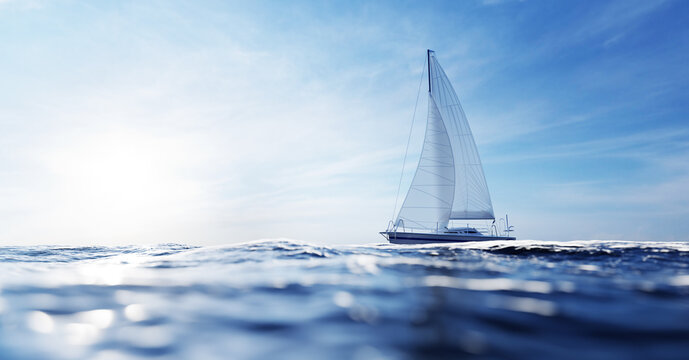
\includegraphics[width=\headerwidth]{background.jpg}
                % Use 'width' alone (no height) to preserve aspect ratio — 
                % the clip will hide the overflow top and bottom.
                % Swap to 'height=\headerheight' if your image is taller than wide.
            };
        \end{scope}

        % Dark overlay for contrast
        \fill[black, opacity=0.3] (0,0) rectangle (\headerwidth, \headerheight);

        % Text on top
        \node[align=center] at (0.5*\headerwidth, 0.5*\headerheight) {
            {\VeryHuge \textcolor{titletext}{#2}}\\[10mm]
            {\Huge \textcolor{titletext}{#3}}\\[10mm]
            {\Large \textcolor{titletext}{#4}}
        };
    \end{tikzpicture}
    \vspace{#1}
}

% Create the fancy subtitle command
\NewDocumentCommand{\FancySubtitle}{ O{1cm} O{1cm} m }{
    \vspace{#2}
    \noindent
    \fcolorbox{subtitleoutline}{subtitlebackground}{\begin{minipage}{\dimexpr\linewidth-2\fboxsep-2\fboxrule\relax}
        \centering
        \sf \huge \textcolor{subtitletext}{#3}
    \end{minipage}}
    \vspace{#1}
}

% Create the fancy figure command
\NewDocumentCommand{\FancyFigure}{ O{0.9} m m m }{
    \begin{center}
        \begin{minipage}{#1\linewidth}
          \centering
          \includegraphics[width=\linewidth]{#2}
          \captionof{figure}{#3}
          \label{#4}
        \end{minipage}
    \end{center}
}

%%%%%%%%%%%%%%%%%%%%%%%%%%%%%%%%%%%%

\begin{document}

\FancyTitle{Go With the Flow:}{Optimizing the 100 Miler Sailing Race}{Connor McBride, Ethan Palenske, and Jackson Pond}

%Main
\color{black}
\noindent
\begin{minipage}{\linewidth + 2\fboxsep}
\begin{multicols*}{\NumColumns}
    \FancySubtitle[5mm]{Overview}
        \begin{center}
            % 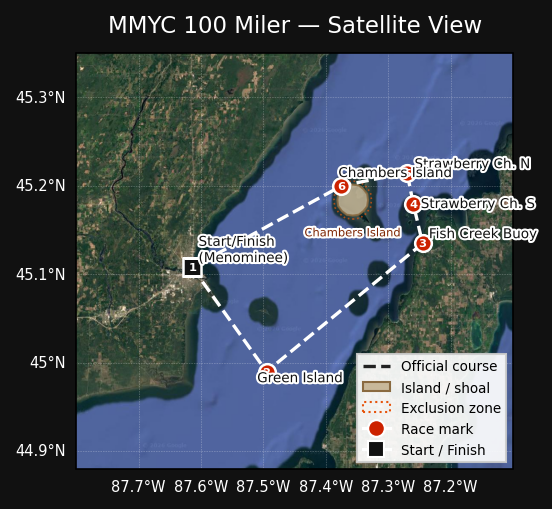
\includegraphics[width=1\linewidth, trim={0 9cm 0 91cm}, clip]{route_map.png}
            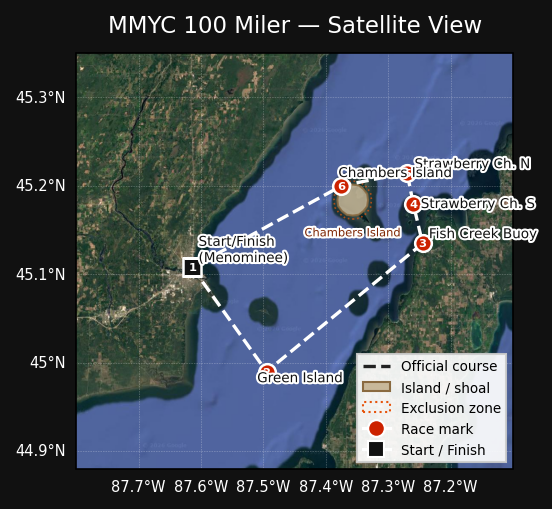
\includegraphics[width=1\linewidth]{route_map.png}
        \end{center}
        
        \large The historic M\&M 100 Miler sailing race takes place annualy in Lake Michigan. In this project we determined the optimal path for a sailboat to take in this race. We use a few different models; a simple one assuming uniform current and wind, a more complex one that accounts for real-world sailing dynamics, and the most advanced one that accounts for variable wind and current. Our goal was to determine the simplest model that would re-discover real world sailing techniques, particularly tacking.

\FancySubtitle[0cm][2cm]{The problem}
    \begin{center}
    \LARGE{\textbf{Assumptions \& Equations}}
    \end{center}
    \vspace{5mm}
        \large As the sun dipped below the horizon, casting hues of orange and pink across the sky, the quaint village came to life with the soft chatter of its inhabitants. Children chased each other through narrow cobblestone streets, their laughter echoing against the ancient stone walls. The scent of freshly baked bread wafted from the local bakery, enticing passersby with its warm embrace. In the distance, the sound of church bells rang out, signaling the end of another peaceful day in this idyllic countryside retreat.

\columnbreak
You could use Tikz to make figures (if you want)

\begin{center}
    \vspace{5mm}
    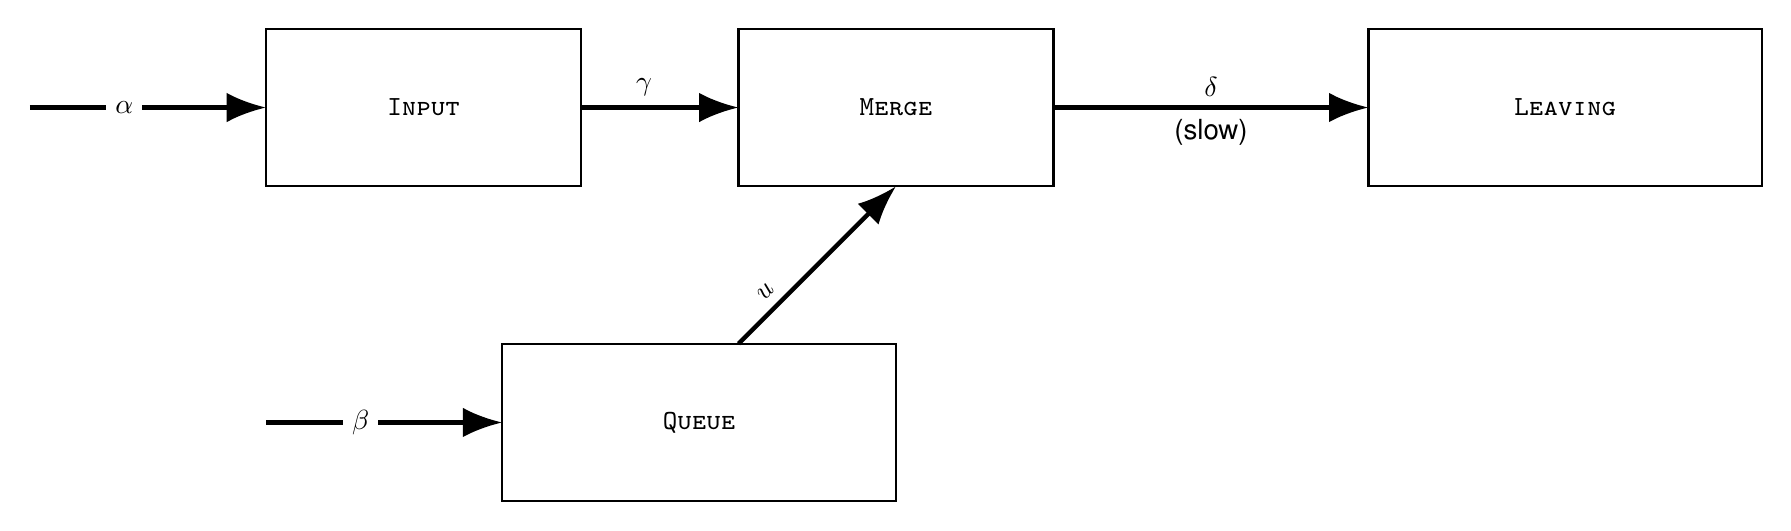
\begin{tikzpicture}
        \draw[thick] (0,0) rectangle ++(4,2) node[midway] {\textsc{\texttt{Input}}};
        \draw[thick] (6,0) rectangle ++(4,2) node[midway] {\textsc{\texttt{Merge}}};
        \draw[thick] (14,0) rectangle ++(5,2) node[midway] {\textsc{\texttt{Leaving}}};
        \draw[thick] (3,-4) rectangle ++(5,2) node[midway] {\textsc{\texttt{Queue}}};
        \draw[-{Latex[length=5mm]}, ultra thick] (-3, 1) -- (0, 1) node[pos=.4, fill=white] {$\alpha$};
        \draw[-{Latex[length=5mm]}, ultra thick] (0, -3) -- (3, -3) node[pos=.4, fill=white] {$\beta$};
        \draw[-{Latex[length=5mm]}, ultra thick] (4, 1) -- (6, 1) node[pos=.4,above] {$\gamma$};
        \draw[-{Latex[length=5mm]}, ultra thick] (10, 1) -- (14, 1) node[midway,above] {$\delta$} node[midway,below] {(slow)};
        \draw[-{Latex[length=5mm]}, ultra thick] (6,-2) -- (8,0) node[near start,sloped,above] {$u$};
    \end{tikzpicture}
    \vspace{5mm}
\end{center}

\begin{center}
\LARGE{\textbf{The approach}}
\end{center}
\large

Describe what you are going to try and accomplish

As the sun dipped below the horizon, casting hues of orange and pink across the sky, the quaint village came to life with the soft chatter of its inhabitants. Children chased each other through narrow cobblestone streets, their laughter echoing against the ancient stone walls. The scent of freshly baked bread wafted from the local bakery, enticing passersby with its warm embrace. In the distance, the sound of church bells rang out, signaling the end of another peaceful day in this idyllic countryside retreat.
            
% \FancyFigure{Figure file}{Figure caption.}{fig:evolution-comparison}

\begin{center}
\vspace{2cm}
\LARGE{\textbf{Another heading}}
\end{center}
\large As the sun dipped below the horizon, casting hues of orange and pink across the sky, the quaint village came to life with the soft chatter of its inhabitants. Children chased each other through narrow cobblestone streets, their laughter echoing against the ancient stone walls. The scent of freshly baked bread wafted from the local bakery, enticing passersby with its warm embrace. In the distance, the sound of church bells rang out, signaling the end of another peaceful day in this idyllic countryside retreat.


\columnbreak
\begin{center}
\LARGE{\textbf{Infinite-Time LQR}}
\end{center}

Only if you actually used Infinite-Time LQR?

As the sun dipped below the horizon, casting hues of orange and pink across the sky, the quaint village came to life with the soft chatter of its inhabitants. Children chased each other through narrow cobblestone streets, their laughter echoing against the ancient stone walls. The scent of freshly baked bread wafted from the local bakery, enticing passersby with its warm embrace. In the distance, the sound of church bells rang out, signaling the end of another peaceful day in this idyllic countryside retreat.


\FancySubtitle[4mm][1cm]{Early Results \& Analysis}

\begin{center}
    % \includegraphics[width=1\linewidth,trim={0 8cm 0 10cm},clip]{anothepicture.png}
\end{center}

As the sun dipped below the horizon, casting hues of orange and pink across the sky, the quaint village came to life with the soft chatter of its inhabitants. Children chased each other through narrow cobblestone streets, their laughter echoing against the ancient stone walls. The scent of freshly baked bread wafted from the local bakery, enticing passersby with its warm embrace. In the distance, the sound of church bells rang out, signaling the end of another peaceful day in this idyllic countryside retreat.


\columnbreak  
As the sun dipped below the horizon, casting hues of orange and pink across the sky, the quaint village came to life with the soft chatter of its inhabitants. Children chased each other through narrow cobblestone streets, their laughter echoing against the ancient stone walls. The scent of freshly baked bread wafted from the local bakery, enticing passersby with its warm embrace. In the distance, the sound of church bells rang out, signaling the end of another peaceful day in this idyllic countryside retreat.

\FancySubtitle[4mm][1cm]{Conclusions and next steps}
As the sun dipped below the horizon, casting hues of orange and pink across the sky, the quaint village came to life with the soft chatter of its inhabitants. Children chased each other through narrow cobblestone streets, their laughter echoing against the ancient stone walls. The scent of freshly baked bread wafted from the local bakery, enticing passersby with its warm embrace. In the distance, the sound of church bells rang out, signaling the end of another peaceful day in this idyllic countryside retreat.

\bibliographystyle{amsalpha}
\bibliography{poster_references}
\end{multicols*}
\end{minipage}

\nocite{unsplash}
%Using nocite allows a reference to appear in the reference list without a citation appearing in the poster.
\footnotesize

\end{document}